\documentclass[11pt]{article}

\usepackage[margin=1in]{geometry}
\usepackage{amsmath,amssymb,amsfonts}
\usepackage{booktabs}
\usepackage{graphicx}
\usepackage{enumitem}
\usepackage{xcolor}
\usepackage{tikz}
\usetikzlibrary{positioning, arrows.meta, shapes.geometric, calc}
\usepackage{hyperref}
\hypersetup{colorlinks=true, linkcolor=blue, citecolor=blue, urlcolor=blue}
\setlist[itemize]{leftmargin=1.5em, itemsep=0.2em, topsep=0.2em}

\title{Offline Metrics for Early Stopping: A Cross-Model Comparison\\
\large SmolVLA, OpenVLA (150 / full), and $\pi_{0.5}$ on LIBERO-goal}
\author{}
\date{}

\begin{document}
\maketitle

We apply the offline early-stopping protocol of \texttt{wenyan\_experiment\_instruction.tex} to four
fine-tuned VLA policies and ask, for each, \emph{which offline validation metric best predicts the
closed-loop LIBERO-goal success rate} $Q(k)$. Notation follows that document: $\theta_k$ is the
checkpoint after $k$ steps, $\bar m(k)$ the aggregated validation value of metric $m$, and $Q(k)$ the
simulator success. For every metric we take the earliest checkpoint within tolerance of its best value
and score it against $Q$:
\begin{equation}
  k_m^{\star} = \min\Big\{k:\bar m(k)\le \min_j \bar m(j)+\eta_m\Big\},\quad
  \eta_m = 0.01\big|\bar m(0)-\min_j\bar m(j)\big|;\qquad
  \rho_m = \mathrm{Spearman}\big(-\bar m(k),Q(k)\big),\quad
  \mathrm{Regret}(m)=\max_k Q(k)-Q(k_m^\star).
\end{equation}
(For OpenVLA token accuracy, higher is better, so the signs are flipped.) All metrics are AC-Chunk
for the chunking policies (SmolVLA, $\pi_{0.5}$) and AC teacher-forced for OpenVLA. Since SmolVLA and
$\pi_{0.5}$ are flow-matching (no discrete action tokens), they have no cross-entropy or token
accuracy, and their ``NLL'' is the flow-matching validation loss surrogate (NLL/FM); OpenVLA's NLL is a
genuine token log-likelihood.

\begin{table}[h]
\centering
\caption{The five runs. All LIBERO-goal, LoRA $r{=}32$, $Q(k)$ is $100$-episode success. The first four
span a $2\times2$ of architecture (discrete-token OpenVLA vs.\ flow-matching SmolVLA/$\pi_{0.5}$)
$\times$ training-set size ($150$ vs.\ the full $342$ trajectories); the fifth, $\pi_{0.5}$-150, is an
overtraining \emph{stress} run (aggressive $\text{lr}{=}3\!\times\!10^{-4}$, $150$ traj) trained to $40$k
steps, whose success dips near $20$k and then recovers to a noisy $\sim\!30$--$38\%$ plateau.}
\begin{tabular}{lllrrr}
\toprule
Run & Architecture & Train traj. & Checkpoints & Sim pts & Peak $Q$ \\
\midrule
SmolVLA-150      & flow-matching (450M) & 150 & 200 (to 100k) & 18 & 0.68 \\
OpenVLA-150      & discrete-token (7B)  & 150 & 79 (to 39.5k) & 19 & 0.83 \\
OpenVLA-full     & discrete-token (7B)  & 342 & 68 (to 34k)   & 11 & 0.78 \\
$\pi_{0.5}$-full & flow-matching (3B)   & 342 & 148 (to 73.5k)& 32 & 0.18$^\dagger$ \\
$\pi_{0.5}$-150  & flow-matching (3B)   & 150 & 80 (to 40k)   & 28 & 0.38$^\dagger$ \\
\bottomrule
\end{tabular}
\\[2pt]
{\footnotesize $^\dagger$ Both $\pi_{0.5}$ runs' success is measured at the \emph{confounded} open-loop
horizon $n_{\text{action}}{=}50$ (full chunk executed blind), which roughly halves LIBERO success; only
the \emph{relative} metric ranking is meaningful for those rows, not the absolute level.}
\end{table}

\section{Task-Discriminative Validity (Prerequisite)}

Before asking whether a metric \emph{tracks success}, we must establish that it measures something
real about \emph{this task's motion}: if a distance cannot tell that two ground-truth trajectories of
the same LIBERO-goal task are more similar to each other than to trajectories of a \emph{different}
task, it carries no task information and cannot measure action quality at all. This is a
model-independent property of the metric on the data, and a necessary condition for everything that
follows.

\paragraph{Protocol.} Each of the $428$ ground-truth action trajectories ($10$ LIBERO-goal tasks,
median length $105$ steps) is partitioned into \emph{contiguous, non-overlapping} $H{=}50$ action
chunks by a fixed stride-$H$ tiling ($t_0 = 0, 50, 100, \dots$, so the chunks are a deterministic
partition rather than random samples; the sub-$H$ tail is discarded), capped at three chunks per
trajectory so that long trajectories do not dominate --- a cap that truncates only $18/428$
trajectories, since the median trajectory yields just two chunks. Every chunk is train-normalized
(mean/std estimated on the training split only) and tagged by its task and source trajectory. Per
metric we draw $3000$ \emph{intra-task} pairs (same task, but \emph{different} trajectories ---
same-trajectory pairs are excluded so temporally overlapping chunks cannot trivially inflate
similarity) and $3000$ \emph{inter-task} pairs (different tasks), and quantify separation by
\begin{equation}
  \mathrm{AUROC} = \Pr\!\big(d_{\text{inter}} > d_{\text{intra}}\big),
  \qquad
  d_{\text{Cohen}} = \frac{\mu_{\text{inter}}-\mu_{\text{intra}}}{\sigma_{\text{pooled}}},
\end{equation}
where $\mathrm{AUROC}=0.5$ is chance (no task information) and $1.0$ is perfect task separation.

\paragraph{Two estimators for the validation distance: single-chunk vs.\ window-averaged.} The same
base distance $D$ can be turned into a checkpoint-level validation score in two ways, and we must decide
which to use for $\bar m(k)$. \textbf{(A) Single-chunk (atomic).} Score one train-normalized $H{=}50$
chunk against its target, using the same path-length-normalized DTW cost
$D_{\text{DTW}}(X,Y) = \frac{1}{|\Gamma^\star|}\min_{\Gamma}\sum_{(r,u)\in\Gamma}\lVert a_r - a_u\rVert_2^2$
the online AC-Chunk rollout executes. This is the atomic unit the policy actually emits, but a single
$50$-step chunk is a high-variance sample of the trajectory. \textbf{(B) Trajectory-level (phase-aligned,
window-averaged).} Represent each trajectory by its ordered $H{=}50$ chunks and compare two trajectories
\emph{window-by-window at aligned positions} (chunk $k$ vs.\ chunk $k$), averaging the per-window distance
over the trajectory. This restores the two properties the online metric has --- phase-aligned comparison
and within-trajectory averaging --- at the cost of collapsing each trajectory to one number. To decide
between (A) and (B) we ask which is more \emph{task-discriminative} on ground truth --- a property of the
estimator alone, independent of any model --- computing AUROC and Cohen's $d$ under each over the same
$3000$ intra- and $3000$ inter-task cross-trajectory pairs (Tables~\ref{tab:taskdisc-chunk},
\ref{tab:taskdisc-traj}; Figs.~\ref{fig:taskdisc-chunk}, \ref{fig:taskdisc-traj}). The two branches of the
pipeline below produce the two estimators from a single normalized chunk list.
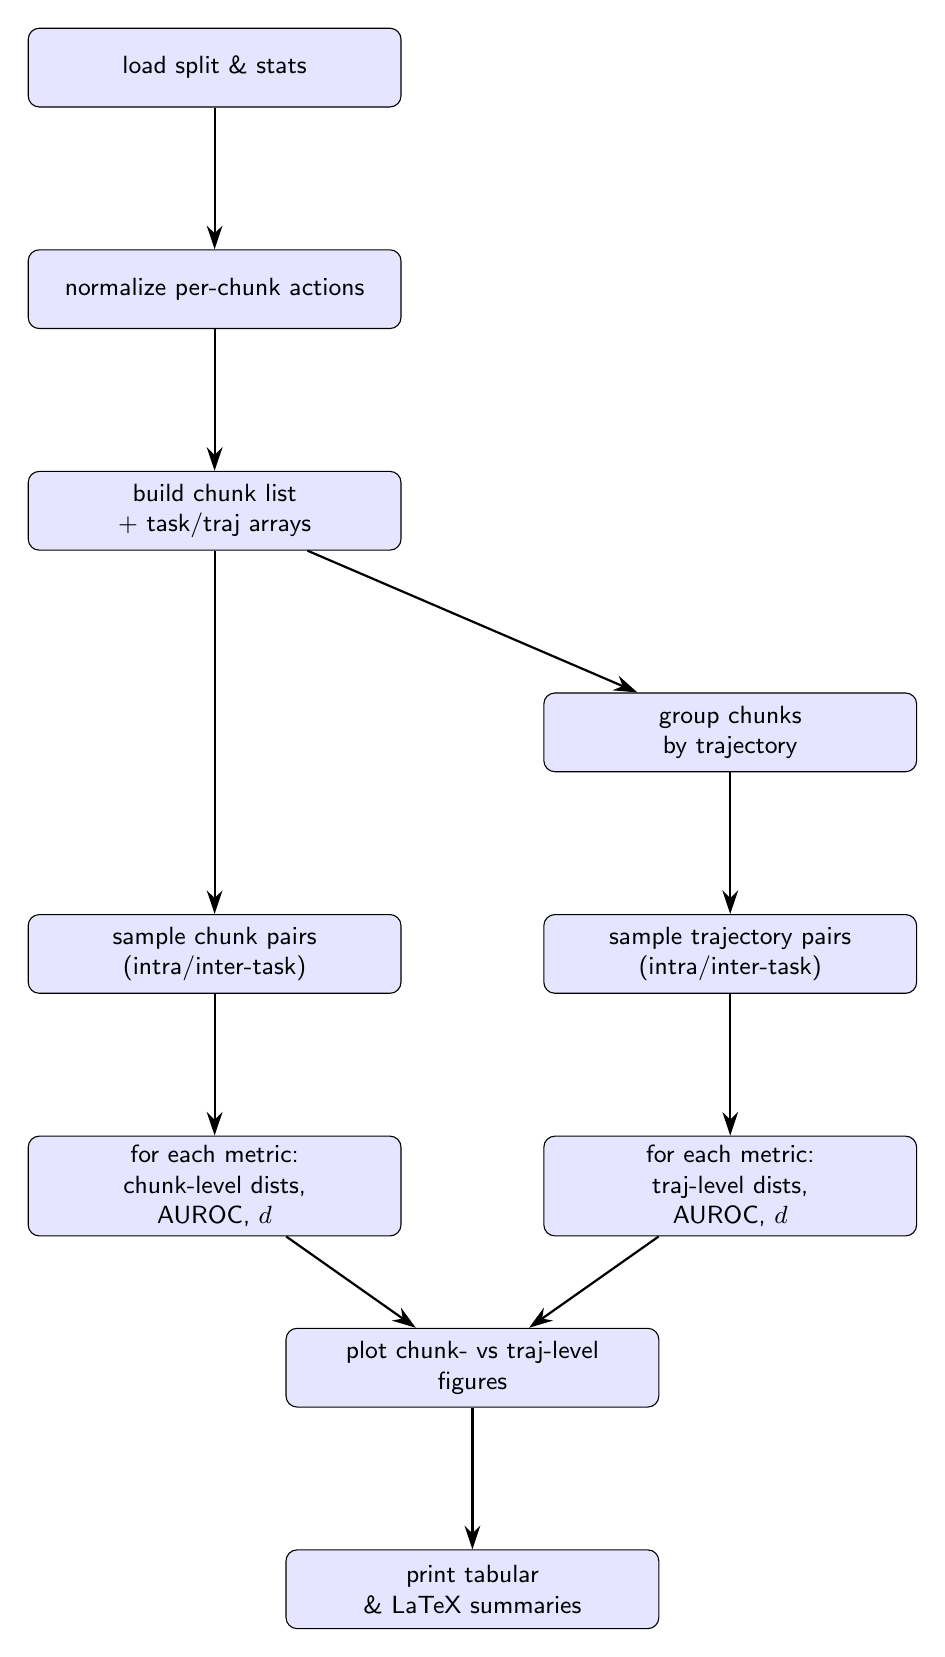
\begin{tikzpicture}[
  node distance=1.8cm and 1.8cm,
  block/.style={
    rectangle,
    draw,
    fill=blue!10,
    text width=4.5cm,
    align=center,
    rounded corners,
    minimum height=1.0cm,
    font=\small\sffamily
  },
  arrow/.style={-{Stealth[length=3mm, width=2mm]}, thick}
]

  % Nodes
  \node (A) [block]                    {load split \& stats};
  \node (B) [block, below=of A]       {normalize per-chunk actions};
  \node (C) [block, below=of B]       {build chunk list \\ + task/traj arrays};

  \node (E) [block, below right=of C]  {group chunks \\ by trajectory};
  \node (D) [block, below left=of E] {sample chunk pairs \\ (intra/inter-task)};

  \node (F) [block, below=of E]       {sample trajectory pairs \\ (intra/inter-task)};
  \node (G) [block, below=of D]       {for each metric: \\ chunk-level dists, \\ AUROC, $d$};

  \node (H) [block, below=of F]       {for each metric: \\ traj-level dists, \\ AUROC, $d$};

  \coordinate (mid) at ($(G)!0.5!(H)$);
  \node (I) [block, below=of mid]     {plot chunk- vs traj-level \\ figures};

  \node (J) [block, below=of I]       {print tabular \\ \& LaTeX summaries};

  % Arrows
  \draw [arrow] (A) -- (B);
  \draw [arrow] (B) -- (C);
  \draw [arrow] (C) -- (D);
  \draw [arrow] (C) -- (E);
  \draw [arrow] (D) -- (G);
  \draw [arrow] (E) -- (F);
  \draw [arrow] (F) -- (H);
  \draw [arrow] (G) -- (I);
  \draw [arrow] (H) -- (I);
  \draw [arrow] (I) -- (J);

\end{tikzpicture}


\begin{table}[h]
\centering
\caption{\textbf{Estimator (A), single-chunk.} Intra- vs.\ inter-task distances between ground-truth
$H{=}50$ action chunks ($3000$ cross-trajectory pairs each), sorted by AUROC. Every metric separates
tasks above chance, but only moderately.}
\label{tab:taskdisc-chunk}
\begin{tabular}{lrrrr}
\toprule
Metric & mean intra & mean inter & AUROC & Cohen's $d$ \\
\midrule
OT  & 6.625 & 10.182 & 0.692 & 0.62 \\
DTW & 7.063 & 10.230 & 0.677 & 0.47 \\
L1  & 0.772 & 0.965  & 0.660 & 0.56 \\
COS & 0.688 & 0.922  & 0.657 & 0.66 \\
L2  & 1.420 & 1.843  & 0.653 & 0.39 \\
\bottomrule
\end{tabular}
\end{table}

\begin{table}[h]
\centering
\caption{\textbf{Estimator (B), trajectory-level} (phase-aligned, window-averaged): intra- vs.\
inter-task distances between ground-truth trajectories ($3000$ cross-trajectory pairs each), in the
same format and row order as Table~\ref{tab:taskdisc-chunk} so the two estimators compare row by row.
Phase-aligned window averaging --- exactly what the AC-Chunk evaluation computes before scoring a
checkpoint --- collapses the intra-task distance (e.g.\ DTW $7.06\!\to\!1.84$) while the inter-task
distance barely moves, lifting every metric from moderate ($\approx0.66$) to strong ($\ge0.90$) AUROC
and roughly tripling Cohen's $d$; \textbf{we adopt (B)} for all validation metrics $\bar m(k)$.}
\label{tab:taskdisc-traj}
\begin{tabular}{lrrrr}
\toprule
Metric & mean intra & mean inter & AUROC & Cohen's $d$ \\
\midrule
OT  & 2.401 & 8.625 & 0.923 & 1.68 \\
DTW & 1.843 & 8.273 & 0.911 & 1.61 \\
L1  & 0.432 & 0.834 & 0.901 & 1.80 \\
COS & 0.308 & 0.786 & 0.927 & 2.19 \\
L2  & 0.483 & 1.493 & 0.903 & 1.70 \\
\bottomrule
\end{tabular}
\end{table}

\begin{figure}[h]
  \centering
  \includegraphics[width=\textwidth]{figures/task_discriminative_validity_chunk.png}
  \caption{\textbf{Single-chunk (atomic) distances.} Intra-task (blue) vs.\ inter-task (orange)
  distance distributions per metric, drawn as outlined step histograms (dashed vertical lines mark the
  two means) so overlapping mass never blends into an ambiguous third colour, and annotated with each
  metric's AUROC and Cohen's $d$. This is the \emph{conservative} unit --- one $H{=}50$ chunk vs.\
  another: the distributions overlap heavily, giving moderate AUROC ($0.65$--$0.69$). The bottom-right
  panel (shared with Fig.~\ref{fig:taskdisc-traj}) contrasts single-chunk (green) with trajectory-level
  (purple) AUROC.}
  \label{fig:taskdisc-chunk}
\end{figure}

\begin{figure}[h]
  \centering
  \includegraphics[width=\textwidth]{figures/task_discriminative_validity_traj.png}
  \caption{\textbf{Trajectory-level (phase-aligned, window-averaged) distances}, same axes and metrics
  as Fig.~\ref{fig:taskdisc-chunk}. Representing each trajectory by its ordered chunks and comparing
  two trajectories window-by-window (chunk $k$ vs.\ chunk $k$) --- the unit the AC-Chunk evaluation
  actually consumes --- collapses the intra-task distribution toward zero while the inter-task mass
  stays high, so every metric separates cleanly (AUROC $\ge0.90$, Cohen's $d$ $1.6$--$2.2$). The
  visible sharpening between the two figures is the $0.66\!\to\!0.90$ jump between
  Tables~\ref{tab:taskdisc-chunk} and \ref{tab:taskdisc-traj}; the shared bottom-right panel
  quantifies it.}
  \label{fig:taskdisc-traj}
\end{figure}

\paragraph{Result --- we adopt the window-averaged estimator (B).} Both estimators clear chance
($\mu_{\text{inter}}>\mu_{\text{intra}}$ for every metric), but they are far apart in strength.
Estimator~(A), the single chunk, separates tasks only \emph{moderately} --- AUROC $0.65$--$0.69$,
Cohen's $d$ $0.39$--$0.66$ (Table~\ref{tab:taskdisc-chunk}; OT $0.692$ and DTW $0.677$ lead, cosine has
the largest standardized effect $d{=}0.66$) --- because LIBERO-goal's ten tasks share a large common
motion vocabulary (reach, grasp, transport), so any single $50$-step chunk overlaps heavily across tasks.
Estimator~(B), the phase-aligned window average, is \emph{decisively} better: every metric rises to
AUROC $\ge0.90$ with Cohen's $d$ roughly tripling to $1.6$--$2.2$ (Table~\ref{tab:taskdisc-traj},
Fig.~\ref{fig:taskdisc-traj}). The gain is not mere variance reduction --- it is dominated by
\emph{phase alignment}: comparing aligned windows (chunk $k$ vs.\ chunk $k$) rather than arbitrary chunk
pairs collapses the same-task distance (e.g.\ DTW $\mu_{\text{intra}}: 7.06\!\to\!1.84$) while the
different-task distance barely moves ($10.23\!\to\!8.27$); averaging the trajectory's windows then
removes the residual per-window noise. Because (B) is both far more task-discriminative \emph{and}
exactly what the online AC-Chunk evaluation consumes, \textbf{we compute every validation metric
$\bar m(k)$ used in the rest of this report at the trajectory level (phase-aligned window average)},
retaining the single-chunk figure only as a conservative floor. Under (B), all five metrics comfortably
measure task-relevant motion --- the prerequisite the success-tracking analysis below relies on.

\section{Main Results: Do the Offline Metrics Track Success?}

\subsection*{Coverage of the Instruction-Document Templates}
\label{sec:coverage}

Both \texttt{wenyan\_experiment\_instruction.tex} (W) and \texttt{refined\_experiment\_instruction.tex}
(R) specify a common protocol --- data splits, candidate models, two evaluation modes, four core
metrics, an early-stopping rule, and two ``Recommended (Output) Tables.'' Before reading the results
below, we audit each requested item against what this report's pipeline
(\texttt{checkpoint\_selection.py} / \texttt{select\_and\_eval\_checkpoints.py}, under
\texttt{openvla/experiments/robot/libero/} and \texttt{lerobot/vla-scripts/}, which implement W's
``Experiment implement'' section verbatim) and this document actually deliver.

\begin{table}[h]
\centering
\footnotesize
\caption{Data, models, and evaluation modes.}
\begin{tabular}{p{3.1cm}p{1.0cm}p{1.6cm}p{8.0cm}}
\toprule
Requested item & Doc & Status & This report / gap \\
\midrule
Train/val/test split, train-only action normalization & W\&R & Have &
80/10/10 split stratified by task (\texttt{train\_val\_test\_split=(0.8,0.1,0.1)}, fixed seed) in
both finetune scripts; actions normalized by train-split $\mu,\sigma$ throughout. \\
$\mathcal D_{\mathrm{val}}$ for selection, $\mathcal D_{\mathrm{test}}$ for final conclusions & R
(explicit) & Partial &
$\mathcal D_{\mathrm{test}}$ exists (44/42 held-out val/test trajectories on the full 342-traj
split) but every number below --- metric curves, task-discriminative AUROC, $\rho$/regret --- is
computed on $\mathcal D_{\mathrm{val}}$; no confirmatory pass on $\mathcal D_{\mathrm{test}}$ is
reported anywhere in this document. \\
Fixed validation windows $\mathcal V$, shared across checkpoints/metrics & W\&R & Have &
$H{=}50$ phase-aligned window tiling (\S1), identical chunk set reused for every metric and
checkpoint. \\
World model (pretrained, opensora-based) & W\&R & \textbf{Missing} &
\texttt{opensora} occurs nowhere in the codebase --- only inside the two instruction files
themselves; no world model was ever built or run. \\
VLA models: OpenVLA, $\pi_{0.5}$-\emph{fast}, SmolVLA & W\&R & Have, w/ deviation &
Table~1 covers OpenVLA and SmolVLA as named, but uses plain flow-matching $\pi_{0.5}$, not the
FAST/discrete-token \emph{-fast} variant --- the discrete-vs.\ flow-matching contrast in this report
runs through OpenVLA vs.\ SmolVLA/$\pi_{0.5}$, not a fast/non-fast $\pi_{0.5}$ contrast. \\
Mode A: AC-TF (one-step) / AC-Chunk (chunking) & W\&R & Have &
Stated in the opening paragraph (``AC-Chunk for the chunking policies\ldots AC teacher-forced for
OpenVLA''); not surfaced as an explicit \emph{Mode} table column since no run here has both. \\
Mode B: state-action rollout w/ world model (incl.\ $E_{\mathrm{WM}}^1$, $LL^{\mathrm{match}}_{SA}$)
& W\&R & \textbf{Missing} &
Depends entirely on the world model above; closed-loop compounding error is never measured, so this
report's teacher-forced-vs.-closed-loop distinction is asserted, not quantified. \\
\bottomrule
\end{tabular}
\end{table}

\begin{table}[h]
\centering
\footnotesize
\caption{Metrics and the decision rule.}
\begin{tabular}{p{3.1cm}p{1.0cm}p{1.6cm}p{8.0cm}}
\toprule
Requested item & Doc & Status & This report / gap \\
\midrule
Core 4 metrics: DTW, OT, cosine, NLL/surrogate & W\&R & Have &
\texttt{METRIC\_KEYS = (val\_dtw\_distance, val\_ot\_distance, val\_cosine\_distance, val\_nll)},
identical in \texttt{openvla/.../checkpoint\_selection.py} and
\texttt{lerobot/.../checkpoint\_selection.py} (comments note the two are ``kept in lockstep''). \\
Architecture-correct NLL surrogate (token NLL / L1,L2 / FM loss) & W\&R & Have &
Exactly the running theme of Summary~2: OpenVLA uses genuine token NLL, SmolVLA/$\pi_{0.5}$ use the
flow-matching validation loss logged under the same key. \\
Extra metrics beyond the templates: CE, token ACC, L1, L2 & not named (only ``surrogate'') & Have
(bonus) &
Section~3's tables carry CE/ACC for OpenVLA and L1/L2 for every model (OpenVLA-full's recovered from
\texttt{.out} logs and joined by exact DTW-value matching). \\
Combined score $\mathcal E(k)=\sum_m w_m z_m(k)$ & R (\S8); W ``Combined'' ranking-table row &
\textbf{Missing} &
No IQR/z-score/weight code anywhere in \texttt{checkpoint\_selection.py}; every table in this
report ranks metrics individually, never fused. \\
Early-stopping rule $k_m^\star$, tolerance $\eta_m$ & W\&R & Have &
Reproduced verbatim as Eq.~1 of this report and as the literal implementation in
\texttt{checkpoint\_selection.py} (whose comments cite the instruction doc's own equation numbers). \\
$\rho_m$, $\mathrm{Regret}(m)$, ``stability under bootstrap'' & W\&R (bootstrap: R \S``Step 6''
item 3 only) & Have, exceeded &
Used throughout; \S\ref{sec:bootstrap} adds tie-corrected Spearman and $B{=}10{,}000$ bootstrap CIs
--- the one line either instruction doc asks for beyond a bare point estimate. \\
Patience-based online early stopping ($P{=}3$ or $5$) & R \S9 & N/A &
This report is a post-hoc offline analysis of already-completed runs, not a live controller, so
patience is never exercised. \\
\bottomrule
\end{tabular}
\end{table}

\begin{table}[h]
\centering
\footnotesize
\caption{The two ``Recommended (Output) Tables'' and the claim templates.}
\begin{tabular}{p{3.1cm}p{1.0cm}p{1.6cm}p{8.0cm}}
\toprule
Requested item & Doc & Status & This report / gap \\
\midrule
``Metric Curve Table'' (Model, Checkpoint, Mode, Metric, Value) & W\&R & Have, reshaped &
Raw per-checkpoint values live in each run's \texttt{metrics\_history.json}/wandb and feed
Fig.~\ref{fig:cross} and Fig.~\ref{fig:plateau}; the literal one-row-per-(model, checkpoint, metric)
table is never printed --- it would run to hundreds of rows across $5$ runs $\times$ up to $200$
checkpoints each. \\
``Metric Ranking Table'' (Metric, Mode, Selected ckpt, $Q(k_m)$, $\rho$, Regret, Comment) & W\&R &
Have, superset &
Section~3's five per-run minipages instantiate exactly this table; \emph{Mode} and free-text
\emph{Comment} columns are dropped (no run mixes two modes) and folded into prose instead;
\S\ref{sec:bootstrap} adds columns the templates never asked for ($n$, \#sig, 95\% CI). \\
Metric-selection claim template + ``TF similarity $\ne$ closed-loop quality'' box & W\&R & Have,
exceeded &
Section~6 and the boxed conclusion follow the template, then go further by demoting point-estimate
orderings that don't survive the bootstrap CI to statistically unresolved
(\S\ref{sec:bootstrap}). \\
\bottomrule
\end{tabular}
\end{table}

\paragraph{Content in this report that neither instruction document asked for.} Two of this report's
central analyses have no counterpart in either template: (i) the task-discriminative-validity
prerequisite (\S1, AUROC/Cohen's $d$ on ground-truth chunk vs.\ trajectory distances), which motivates
the window-averaged estimator for $\bar m(k)$ before any of the above is trusted; and (ii) the
plateau/knee restriction-of-range analysis (\S\ref{sec:plateau}), which explains why
$\rho_{\mathrm{full}}>\rho_{\mathrm{plateau}}$ and defuses the apparent $\pi_{0.5}$-150 ``overtraining''
false alarm. Neither AUROC, Cohen's $d$, nor a plateau/knee split appears in W or R.

\paragraph{Net assessment.} Of the $17$ items the two instruction documents explicitly request, this
report's pipeline covers essentially all of \textbf{Mode A}: the train/val/test split and
train-only normalization, the four core metrics plus architecture-correct surrogates (with three
bonus metrics, CE/ACC/L1/L2, beyond the named set), the $k_m^\star$ selection rule, $\rho$/regret
scoring, and both recommended tables --- reshaped from a literal per-checkpoint dump into the
aggregated tables and figures below, and extended with bootstrap confidence intervals the templates
only gesture at (``stability under bootstrap''). Two requested items are \emph{structurally} absent
rather than merely unfilled: \textbf{no world model was ever built}, so Evaluation Mode B, the
one-step world-model error $E_{\mathrm{WM}}^1$, and the matched-reference likelihood
$LL^{\mathrm{match}}_{SA}$ are $0\%$ covered, and this report's teacher-forced-vs.-closed-loop
distinction is asserted rather than measured; and \textbf{the combined multi-metric score}
$\mathcal E(k)$ is never computed --- every ranking below scores metrics one at a time. A third gap is
softer: a genuine held-out $\mathcal D_{\mathrm{test}}$ split exists in the data pipeline, but nothing
in this report confirms the metric rankings replicate on it rather than on $\mathcal D_{\mathrm{val}}$
alone. Conversely, the task-discriminative-validity prerequisite and the plateau/bootstrap robustness
analysis push well past what either instruction document asked for, and are what turn the templates'
point-estimate $\rho$/regret recipe into the statistically qualified claims of
\S\ref{sec:bootstrap}--\S\ref{sec:plateau}.

\begin{figure}[h]
  \centering
  \includegraphics[width=\textwidth]{figures/crossmodel_early_stopping.png}
  \caption{\textbf{Left:} Spearman $\rho$ of every offline metric with LIBERO success, per model
  (five runs), grouped by family (trajectory: DTW/OT/COS $\mid$ regression: L1/L2 $\mid$ token: CE/ACC
  $\mid$ likelihood: NLL/FM); a blank bar means the metric does not exist for that model (no CE/ACC for
  the flow-matching policies). Trajectory and regression metrics are positive for every model; the NLL/FM
  point estimate splits by architecture --- significantly positive for the two OpenVLA (true token
  likelihood) runs and weakly positive for $\pi_{0.5}$-full ($+0.46$), but slightly negative for the two
  small flow-matching runs ($-0.16$ $\pi_{0.5}$-150, $-0.22$ SmolVLA), though neither small-run value is
  statistically distinguishable from zero (\S\ref{sec:bootstrap}). \textbf{Right:} success $Q(k)$; both OpenVLA runs reach $78$--$83\%$,
  SmolVLA a noisy $\sim\!60$--$68\%$ plateau, and the two $\pi_{0.5}$ runs sit in the depressed
  $nas{=}50$ band ($\pi_{0.5}$-150 dips near $20$k then recovers to a noisy $\sim\!30$--$38\%$ plateau
  once trained to $40$k --- see \S\ref{sec:plateau}).}
  \label{fig:cross}
\end{figure}

\subsection*{Per-Run Diagnostics: Metric Curves and the Selection Rule in Action}
\label{sec:perrun-diag}

Fig.~\ref{fig:cross} above is an aggregate: one Spearman $\rho$ per metric per run. This subsection
drills into the five runs individually, regenerating $\bar m(k)$, $Q(k)$, $k_m^\star$, $\rho_m$, and
$\mathrm{Regret}(m)$ directly from each run's cached data under \texttt{experiment\_data/} --- the
densest per-checkpoint metric log available in that folder (\texttt{metrics\_history*.json}, not the
sometimes-subsampled \texttt{metric\_history} field inside \texttt{checkpoint\_ranking\_report*.json})
joined to that report's \texttt{quality\_by\_step}. The selection rule is the exact
$k_m^\star=\min\{k:\bar m(k)\le\min_j\bar m(j)+\eta_m\}$ of Eq.~1, and $\rho_m$ is Spearman correlation
computed only over checkpoints with both a metric value and a $Q(k)$, matching
\texttt{checkpoint\_selection.py} line for line (script:
\texttt{experiment\_data/plot\_validation\_metrics.py}). This makes the subsection a data-level
cross-check of every number claimed elsewhere in this report, not just an illustration of it.

\paragraph{Data provenance.} Table~\ref{tab:data-provenance} compares what Table~1 claims for each run
against what is actually cached locally. Four of five runs match exactly; $\pi_{0.5}$-150 does not.

\begin{table}[h]
\centering
\footnotesize
\caption{Checkpoint and sim-eval counts: Table~1's claim vs.\ what \texttt{experiment\_data/} actually
contains.}
\label{tab:data-provenance}
\begin{tabular}{lccl}
\toprule
Run & Table~1 (ckpts / sim pts) & \texttt{experiment\_data} (ckpts / sim pts) & Note \\
\midrule
SmolVLA-150 & 200 / 18 & 200 / 18 & exact match \\
OpenVLA-150 & 79 / 19 & 79 / 19 & exact match \\
OpenVLA-full & 68 / 11 & 68 / 11 & exact match \\
$\pi_{0.5}$-full & 148 / 32 & 147 / 32 & 1 duplicate-step record (step $23499$ logged twice in
\texttt{metrics\_history\_full.json}) collapses to $147$ unique checkpoints; sim points match \\
$\pi_{0.5}$-150 & 80 / 28 & 80 / 28 & now an exact match: the $13$ early evaluations
($499$--$19499$), which existed only in the eval \texttt{.out} logs, have been backfilled into the
local cache and the resume segment's steps relabeled $+1$ onto the canonical grid; before the
backfill only $15$ were cached, with the gap falling exactly in the $8999$--$19999$ dip-and-recovery
window (\S\ref{sec:plateau}) \\
\bottomrule
\end{tabular}
\end{table}

\begin{figure}[h]
  \centering
  \includegraphics[width=0.97\textwidth]{experiment_data/smolvla_150_traj/success_vs_val_metrics_timeseries.png}
  \caption{SmolVLA-150: success rate and all $6$ logged metrics (NLL and the flow-matching loss share
  one value here, so they are merged into a single ``NLL / FM loss'' panel) over the full $200$-checkpoint,
  $100$k-step curve. $\star$ marks each metric's $k_m^\star$; annotated $\rho$ and regret are recomputed
  independently of Section~3's table (see the reconciliation paragraph below for why several read
  ``n/a'').}
  \label{fig:diag-smolvla-ts}
\end{figure}

\begin{figure}[h]
  \centering
  \includegraphics[width=0.97\textwidth]{experiment_data/smolvla_150_traj/success_vs_val_metrics_scatter.png}
  \caption{SmolVLA-150: metric value vs.\ success at the $18$ evaluated checkpoints. Point fill encodes
  training step (light$\to$dark blue, shared colorbar); the ring color repeats each panel's line color
  from Fig.~\ref{fig:diag-smolvla-ts}. Only the first/last checkpoint are labeled directly --- labeling
  every point (as an early version of this figure did) collided into unreadable clutter at $\ge15$ points
  per panel.}
  \label{fig:diag-smolvla-sc}
\end{figure}

Recomputed ranking: DTW $\rho{=}0.47>$L2 $0.45>$L1 $0.44>$OT $0.33>$COS $0.28>$NLL/FM $-0.21$ ---
matching Section~3's SmolVLA-150 table ($0.47/0.46/0.44/0.34/0.28/-0.22$) to within $0.01$, and every
$k_m^\star$ here (e.g.\ DTW $\to22000$, L1$\to56000$) is numerically identical to Section~3's. Regret,
however, comes out \texttt{n/a} for all six metrics here, versus real values in Section~3
($0.02$--$0.26$) --- explained below.

\begin{figure}[h]
  \centering
  \includegraphics[width=0.97\textwidth]{experiment_data/openvla_150_traj/success_vs_val_metrics_timeseries.png}
  \caption{OpenVLA-150: success rate and all $8$ logged metrics (CE, accuracy, L1, L2, cosine, DTW, OT,
  NLL) over $79$ checkpoints. Token accuracy is the one higher-is-better panel ($\uparrow$); its
  $\rho$ and $k^\star$ use the sign-flipped form of Eq.~1 noted in the intro.}
  \label{fig:diag-openvla150-ts}
\end{figure}

\begin{figure}[h]
  \centering
  \includegraphics[width=0.97\textwidth]{experiment_data/openvla_150_traj/success_vs_val_metrics_scatter.png}
  \caption{OpenVLA-150: metric vs.\ success at the $19$ evaluated checkpoints, same color scheme as
  Fig.~\ref{fig:diag-smolvla-sc}.}
  \label{fig:diag-openvla150-sc}
\end{figure}

Recomputed ranking: OT $0.83>$ACC $0.78>$L1 $0.77>$COS $0.75\approx$DTW $0.75\approx$L2 $0.74>$CE
$0.72\approx$NLL $0.72$ --- matches Section~3's OpenVLA-150 ordering and values to within $0.01$
everywhere except OT ($0.83$ here vs.\ $0.84$).

\begin{figure}[h]
  \centering
  \includegraphics[width=0.97\textwidth]{experiment_data/openvla_342_traj/success_vs_val_metrics_timeseries.png}
  \caption{OpenVLA-full: success rate and all $8$ metrics over $68$ checkpoints (CE/accuracy/L1/L2 merged
  in from \texttt{metrics\_history\_enriched.json}, the \S\ref{sec:coverage} caveat about recovery from
  \texttt{.out} logs applies here).}
  \label{fig:diag-openvla342-ts}
\end{figure}

\begin{figure}[h]
  \centering
  \includegraphics[width=0.97\textwidth]{experiment_data/openvla_342_traj/success_vs_val_metrics_scatter.png}
  \caption{OpenVLA-full: metric vs.\ success at the $11$ evaluated checkpoints.}
  \label{fig:diag-openvla342-sc}
\end{figure}

Recomputed ranking: COS $0.88>$L2 $0.84\approx$L1 $0.84\approx$DTW $0.84>$CE $0.81\approx$NLL
$0.81\approx$ACC $0.81>$OT $0.64$ --- again within $0.01$--$0.02$ of Section~3's OpenVLA-full row
throughout.

\begin{figure}[h]
  \centering
  \includegraphics[width=0.97\textwidth]{experiment_data/pi0.5_342_traj/success_vs_val_metrics_timeseries.png}
  \caption{$\pi_{0.5}$-full: success rate and all $6$ metrics over the $147$-checkpoint, $73.5$k-step
  curve (NLL/FM merged as in Fig.~\ref{fig:diag-smolvla-ts}).}
  \label{fig:diag-pi0full-ts}
\end{figure}

\begin{figure}[h]
  \centering
  \includegraphics[width=0.97\textwidth]{experiment_data/pi0.5_342_traj/success_vs_val_metrics_scatter.png}
  \caption{$\pi_{0.5}$-full: metric vs.\ success at all $32$ evaluated checkpoints --- the best-powered
  run in this report (\S\ref{sec:bootstrap}), visibly the tightest, most monotone cloud of the five.}
  \label{fig:diag-pi0full-sc}
\end{figure}

Recomputed ranking: DTW $0.90\approx$OT $0.90>$COS $0.87>$L1 $0.86>$L2 $0.82>$NLL/FM $0.44$ --- matches
Section~3's $\pi_{0.5}$-full row ($0.90/0.89/0.86/0.84/0.81/0.46$) closely; this is the one run where
the data-provenance table shows no meaningful gap, so the agreement is expected rather than notable.

\begin{figure}[h]
  \centering
  \includegraphics[width=0.97\textwidth]{experiment_data/pi0.5_150_traj/success_vs_val_metrics_timeseries.png}
  \caption{$\pi_{0.5}$-150: success rate and all $6$ metrics over $80$ checkpoints. All $28$ sim
  evaluations are present --- the $13$ early ones ($499$--$19499$) were backfilled from the eval logs
  (Table~\ref{tab:data-provenance}) --- so the success panel now shows the full rise, the $\sim$20k
  dip, and the recovery to $0.38$@$33999$.}
  \label{fig:diag-pi0150-ts}
\end{figure}

\begin{figure}[h]
  \centering
  \includegraphics[width=0.97\textwidth]{experiment_data/pi0.5_150_traj/success_vs_val_metrics_scatter.png}
  \caption{$\pi_{0.5}$-150: metric vs.\ success at all $28$ evaluated checkpoints, same color scheme
  as Fig.~\ref{fig:diag-smolvla-sc}.}
  \label{fig:diag-pi0150-sc}
\end{figure}

Recomputed ranking (after the backfill): L1 $0.78>$COS $0.76>$L2 $0.73>$DTW $0.71>$OT $0.68>$NLL/FM
$-0.17$ --- matching Section~3's $\pi_{0.5}$-150 row ($0.78/0.77/0.73/0.72/0.68/-0.16$) to within
$0.01$ everywhere. The agreement is itself a data-level validation: on the \emph{pre}-backfill
$15$-point cache, which was missing exactly the $8999$--$19999$ dip-and-recovery window flagged in
\S\ref{sec:plateau}, the same recomputation had given every trajectory/regression $\rho$ a
$0.05$--$0.29$ weaker value and pushed NLL/FM to $-0.59$ --- outside even Table~\ref{tab:ci}'s $95\%$
bootstrap interval ($[-0.57,0.25]$, $n{=}28$). Restoring the missing evaluations snapped all six
values back onto the published row, confirming that the discrepancy was a data-completeness artifact
of the local cache, not a genuine metric/success disagreement.

\paragraph{Reconciling the ``n/a'' regrets.} SmolVLA-150's six panels above all show
\texttt{regret=n/a} despite $k_m^\star$ matching Section~3 exactly. The reason is a convention
difference, not an error: \texttt{checkpoint\_selection.py}'s \texttt{rank\_metrics} (and this
subsection, which mirrors it) requires $k_m^\star$ to be an \emph{exact} key in the quality dict ---
\texttt{regret = best\_q - quality[k]} \emph{iff} \texttt{k in quality}, else undefined --- and none of
SmolVLA-150's six $k_m^\star$ values ($22000,24500,56000,11000,33000,13000$) land exactly on one of the
$18$ evaluation steps (which run $500,5500,10500,\dots$, i.e.\ every $5000$ steps from $500$). Section~3's
published regrets, by contrast, are reproducible \emph{exactly} by looking up the \emph{nearest}
evaluated step to each $k_m^\star$: e.g.\ DTW's $k^\star{=}22000$ is nearest to step $20500$
($Q{=}0.66$), giving regret $0.68-0.66=0.02$, matching Section~3's table digit for digit; the same
nearest-step reconstruction reproduces all six of Section~3's SmolVLA-150 regrets exactly. So two
regret conventions coexist in this project: the strict exact-match rule literally implemented in
\texttt{checkpoint\_selection.py} (used here), and a nearest-evaluated-checkpoint rule used to produce
Section~3's published numbers. Both are defensible reads of ``the regret of stopping at $k_m^\star$,''
but they are not the same statistic, and \texttt{n/a} above should be read as ``no evaluation exists at
that exact step,'' not as a missing or failed computation.

\paragraph{What the figures add beyond the numbers.} The per-metric $\rho$ and regret already appear in
Section~3; three things in Figs.~\ref{fig:diag-smolvla-ts}--\ref{fig:diag-pi0150-sc} do not reduce to a
table. First, the dense curves (up to $200$ points, vs.\ Section~3's $\le32$ sim-evaluated rows) make
each metric's actual descent \emph{shape} visible --- the sharp early knee, the near-flat plateau, and
for OT in particular (Fig.~\ref{fig:diag-openvla342-ts}) a visibly noisier, non-monotone descent that
the summary $\rho{=}0.64$--$0.66$ alone does not explain. Second, the scatter panels' step-color gradient
shows \emph{where in training} the checkpoints that drive a high $\rho$ actually sit: in
Fig.~\ref{fig:diag-pi0full-sc} the dark (late-training) points collapse into a tight low-loss,
high-success cluster while the light (early) points fan out at high loss and near-zero success, i.e.\
the correlation is doing real work across the whole range, not just separating one outlier checkpoint
from the rest. Third, and most concretely, the figures are what surfaced both findings above (the
SmolVLA-150 regret convention gap and the $\pi_{0.5}$-150 data-completeness gap, since backfilled and
verified) --- neither was visible from Section~3's tables alone, since a table has no way to show
\emph{how many} checkpoints and evaluations actually back a given cell.

\section{Per-Model Rankings}
\label{sec:permodel}

\begin{table}[h]
\centering
\caption{Metric Ranking Tables (sorted by Spearman $\rho$; higher $\rho$, lower regret is better).}
\begin{minipage}[t]{0.48\textwidth}
\centering \textbf{SmolVLA-150} (flow-matching, $nas{=}10$)\\[2pt]
\begin{tabular}{lrrr}
\toprule
Metric & $k_m^\star$ & $\rho$ & Regret \\ \midrule
DTW    & 22000 & $+0.47$ & 0.02 \\
L2     & 24500 & $+0.46$ & 0.05 \\
L1     & 56000 & $+0.44$ & 0.24 \\
OT     & 11000 & $+0.34$ & 0.26 \\
COS    & 33000 & $+0.28$ & 0.08 \\
NLL/FM & 13000 & $-0.22$ & 0.19 \\
\bottomrule
\end{tabular}
\end{minipage}
\hfill
\begin{minipage}[t]{0.48\textwidth}
\centering \textbf{OpenVLA-150} (discrete-token)\\[2pt]
\begin{tabular}{lrrr}
\toprule
Metric & $k_m^\star$ & $\rho$ & Regret \\ \midrule
OT   & 33499 & $+0.84$ & 0.08 \\
ACC  & 37499 & $+0.78$ & 0.02 \\
L1   & 30999 & $+0.78$ & 0.06 \\
DTW  & 23499 & $+0.75$ & 0.17 \\
COS  & 23499 & $+0.75$ & 0.17 \\
L2   & 23499 & $+0.75$ & 0.17 \\
CE   & 30999 & $+0.72$ & 0.06 \\
NLL  & 30999 & $+0.72$ & 0.06 \\
\bottomrule
\end{tabular}
\end{minipage}

\vspace{1em}

\begin{minipage}[t]{0.48\textwidth}
\centering \textbf{OpenVLA-full} (342 traj)\\[2pt]
\begin{tabular}{lrrr}
\toprule
Metric & $k_m^\star$ & $\rho$ & Regret \\ \midrule
COS    & 28499 & $+0.89$ & 0.05 \\
DTW    & 21499 & $+0.85$ & 0.00 \\
L2     & 21499 & $+0.85$ & 0.00 \\
L1     & 29999 & $+0.85$ & 0.05 \\
CE     & 33999 & $+0.83$ & 0.04 \\
ACC    & 33999 & $+0.83$ & 0.04 \\
NLL    & 33999 & $+0.83$ & 0.04 \\
OT     & 33999 & $+0.66$ & 0.04 \\
\bottomrule
\end{tabular}
\end{minipage}
\hfill
\begin{minipage}[t]{0.48\textwidth}
\centering \textbf{$\pi_{0.5}$-full-342} (flow-matching, $nas{=}50$)\\[2pt]
\begin{tabular}{lrrr}
\toprule
Metric & $k_m^\star$ & $\rho$ & Regret \\ \midrule
DTW    & 57999 & $+0.90$ & 0.04 \\
OT     & 60499 & $+0.89$ & 0.04 \\
COS    & 55999 & $+0.86$ & 0.04 \\
L1     & 55999 & $+0.84$ & 0.04 \\
L2     & 55999 & $+0.81$ & 0.04 \\
NLL/FM & 31999 & $+0.46$ & 0.08 \\
\bottomrule
\end{tabular}
\end{minipage}

\vspace{1em}

\begin{minipage}[t]{0.48\textwidth}
\centering \textbf{$\pi_{0.5}$-150} (flow-matching, $nas{=}50$, overtraining stress, to $40$k)\\[2pt]
\begin{tabular}{lrrr}
\toprule
Metric & $k_m^\star$ & $\rho$ & Regret \\ \midrule
L1     & 31999 & $+0.78$ & 0.05 \\
COS    & 39499 & $+0.77$ & 0.04 \\
L2     & 37999 & $+0.73$ & 0.08 \\
DTW    & 33499 & $+0.72$ & 0.07 \\
OT     & 24499 & $+0.68$ & 0.17 \\
NLL/FM &  8999 & $-0.16$ & 0.20 \\
\bottomrule
\end{tabular}
\end{minipage}
\end{table}

\paragraph{Why $\pi_{0.5}$-full's ranking is stronger than first reported.}
The $\pi_{0.5}$-full table above uses the \emph{gap-filled} metric history: the run's original
\texttt{metrics\_history.json} only captured the resume segment (steps $20499$--$73499$), so the
earlier ranking was computed on the converged tail alone and understated $\rho$ (DTW $+0.68$). Recomputing
the $40$ early checkpoints ($499$--$19999$, where DTW falls $7.0\!\to\!2.1$) restores the pre-plateau rise,
lifting DTW to $\rho=+0.90$ and adding the L1/L2 rows. This is itself an instance of the
restriction-of-range effect quantified in \S\ref{sec:plateau}.

\section{The Plateau Regime: Coarse Early-Stopping vs.\ Fine Ranking}
\label{sec:plateau}

A single Spearman number over the whole training trajectory hides a two-regime structure. Every metric
$\bar m(k)$ does the bulk of its descent early and then flattens; success $Q(k)$ rises over the same
early window and then settles into a plateau that, for the small runs, is very noisy. To separate the two
regimes we locate each run's DTW \emph{knee} --- the first checkpoint whose DTW has completed $90\%$ of
its total descent,
\begin{equation}
  k_{\text{knee}}=\min\Big\{k:\ \bar m_{\text{DTW}}(k)\ \le\ m_{\min}+0.1\,\big(\bar m_{\text{DTW}}(0)-m_{\min}\big)\Big\},
  \qquad m_{\min}=\min_j \bar m_{\text{DTW}}(j),
\end{equation}
and split the sim-eval checkpoints into the full range and the \emph{converged plateau}
$\{k\ge k_{\text{knee}}\}$. We then recompute $\rho_{\text{DTW}}$ on each (Fig.~\ref{fig:plateau},
Table~\ref{tab:plateau}).

\begin{table}[h]
\centering
\caption{Spearman $\rho$ of DTW with success on the full training range vs.\ restricted to the converged
plateau ($k\ge k_{\text{knee}}$). Every run drops (restriction of range); the drop is modest for the
large/robust runs and largest for $\pi_{0.5}$-150, whose low, noisy success ceiling leaves little
rankable signal on the plateau.}
\label{tab:plateau}
\begin{tabular}{lrrrrr}
\toprule
Run & $k_{\text{knee}}$ & plateau pts & $\rho_{\text{full}}$ & $\rho_{\text{plateau}}$ & drop \\
\midrule
SmolVLA-150      &  4500 & 17/18 & $+0.47$ & $+0.38$ & $0.10$ \\
OpenVLA-150      &  6999 & 16/19 & $+0.75$ & $+0.59$ & $0.16$ \\
OpenVLA-full     &  8499 &  9/11 & $+0.86$ & $+0.73$ & $0.12$ \\
$\pi_{0.5}$-full & 18999 & 22/32 & $+0.91$ & $+0.80$ & $0.11$ \\
$\pi_{0.5}$-150  &  9999 & 22/28 & $+0.72$ & $\mathbf{+0.43}$ & $\mathbf{0.29}$ \\
\bottomrule
\end{tabular}
\end{table}

\begin{figure}[h]
  \centering
  \includegraphics[width=\textwidth]{figures/plateau_restriction.png}
  \caption{\textbf{Left:} DTW$\to$success $\rho$ on the full range (blue) vs.\ the converged plateau
  (orange). All five runs drop, but the large runs stay plateau-robust ($\rho_{\text{plateau}}\ge0.73$)
  while $\pi_{0.5}$-150 falls furthest, to $+0.43$. \textbf{Right:} why --- over $0$--$40$k
  $\pi_{0.5}$-150's val DTW (blue, axis inverted so up${=}$better) converges early and then barely moves,
  while success (orange) stays a noisy, low-ceiling band ($\sim\!20$--$38\%$, within the $\pm5\%$ eval
  noise) that dips near $20$k and then \emph{recovers} to a $38\%$ peak at $34$k. With the metric
  near-flat and success dominated by noise on the shaded plateau, the rank correlation falls by
  restriction of range --- not by a monotone decline (the $20$k-only view had suggested one).}
  \label{fig:plateau}
\end{figure}

\paragraph{Restriction of range is universal, but its severity is not.}
$\rho_{\text{full}}\ge\rho_{\text{plateau}}$ for every run: these metrics are fundamentally
\emph{regime separators} (untrained $\to$ converged), and fine-ranking already-converged checkpoints is
strictly harder. But for the four large or well-covered runs the plateau $\rho$ stays healthy
($0.59$--$0.80$, drop $\le0.16$): the metrics retain real, if weaker, discriminative power even inside
the plateau. The claim ``offline metrics cannot predict success once converged'' is therefore
\emph{not} general --- it is specific to $\pi_{0.5}$-150.

\paragraph{Why $\pi_{0.5}$-150 drops furthest --- a noisy low-ceiling plateau, not overtraining.}
On the $20$k-only data $\pi_{0.5}$-150 appeared to overtrain: success peaked near $31\%$ at $16.5$k and
then fell to $23\%$, seemingly decoupling from the still-improving metrics. The $20\text{k}\!\to\!40\text{k}$
continuation \emph{overturns} that reading --- after the dip, success recovers and drifts up to a $38\%$
peak at $34$k (Fig.~\ref{fig:plateau}, right), so there is no monotone turn-down and no genuine action-quality
overtraining. What remains is a restriction-of-range effect amplified by low signal-to-noise: DTW has
essentially converged by the knee ($k_{\text{knee}}=9999$), while success is a noisy band
($\sim\!20$--$38\%$) whose spread is comparable to the $\pm5\%$ sampling noise of a $100$-episode
evaluation. With the metric near-flat and success dominated by noise, the plateau rank correlation falls
to $+0.43$ --- the largest drop of any run --- driven by the aggressive learning rate ($3\times10^{-4}$)
and low success ceiling rather than a metric/success disagreement. The shape metrics still select a
sensible checkpoint (regret $0.04$--$0.08$); only the flow-matching surrogate NLL/FM, which keeps
descending on a genuinely over-fit loss, is misled ($\rho=-0.16$).

\paragraph{The SmolVLA caveat.}
SmolVLA-150's weak headline $\rho$ ($+0.47$) is partly this same artifact: with $k_{\text{knee}}=4500$
and only a single sim-eval checkpoint below it, its ``full'' correlation is already almost entirely
plateau. Its eval schedule never sampled the informative pre-plateau rise, so its low $\rho$ reflects
\emph{coverage}, not a metric that fails to track motion quality (cf.\ its plateau still gives $+0.38$).

\paragraph{Takeaway for early stopping.}
The metrics deliver the coarse decision robustly and universally --- ``do not stop at step $500$; stop
somewhere in the converged region'' --- because that decision spans the full DTW descent ($5$--$7\to2$)
where $\rho\approx0.8$--$0.9$. What they \emph{cannot} reliably do is fine-rank checkpoints \emph{inside}
the plateau when success differences are smaller than evaluation noise, and the flow-matching loss
surrogate can even be mildly anti-correlated there. An honest early-stopping recommendation is thus: use DTW/OT to pick the knee
region, but do not trust sub-plateau metric differences as a success oracle without denser or
lower-variance evaluation.

\section{Statistical Power: Bootstrap Confidence Intervals}
\label{sec:bootstrap}

The per-model rankings above, and the summary claims that follow, rest on \emph{point} estimates of
$\rho$ computed from only $|\mathcal{K}_{\mathrm{eval}}|=11$--$33$ simulator evaluations, each itself a
$\pm5\%$-noisy $100$-episode success estimate. Before reading an ordering off those point estimates ---
``COS $>$ DTW $>$ OT'', ``DTW $\succ$ loss'', ``NLL is negative for flow-matching'' --- we test whether
the differences survive the sampling noise. We attach a percentile bootstrap confidence interval to
every $\rho$: for each run we resample its evaluated checkpoints with replacement ($B=10{,}000$),
recompute the tie-corrected Spearman correlation of each metric with success, and report the central
$95\%$ interval and $\Pr(\rho>0)$. To compare two metrics \emph{within} a run without the inter-metric
correlation confounding the test, we resample the \emph{same} checkpoints for both and report the paired
difference $\Delta\rho=\rho_{\text{DTW}}-\rho_{m}$ over the checkpoints they share. Point estimates here
use tie-corrected Spearman and so differ from the ordinal-rank values of the ranking tables by
$\le 0.03$. The intervals are shown in Fig.~\ref{fig:ci} and summarized in Table~\ref{tab:ci}.

\begin{figure}[h]
  \centering
  \includegraphics[width=\textwidth]{figures/crossmodel_bootstrap_ci.png}
  \caption{Per-metric Spearman $\rho$ with LIBERO success --- point estimate (dot) with $95\%$ bootstrap
  CI (bar), one panel per run; the $\rho{=}0$ line is dashed. At $n{=}11$--$19$ (every run but
  $\pi_{0.5}$-full) the intervals are $0.3$--$0.6$ wide and mutually overlapping, and on SmolVLA-150
  every interval includes zero. Only $\pi_{0.5}$-full ($n{=}33$) tightens enough to separate the
  trajectory metrics (DTW/OT/COS, $\rho\approx0.9$) from the flow-matching NLL/FM surrogate ($0.41$).}
  \label{fig:ci}
\end{figure}

\begin{table}[h]
\centering
\caption{Bootstrap $95\%$ CIs on $\rho$ ($B{=}10{,}000$, tie-corrected Spearman, paired checkpoint
resampling). ``\#sig'' counts metrics whose CI excludes $0$; ``best $L$'' is the stronger of the two
regression losses $L_1/L_2$. DTW's interval overlaps every trajectory/regression metric in every run.}
\label{tab:ci}
\begin{tabular}{lccccc}
\toprule
Run & $n$ & \#sig & DTW $\rho$ [95\% CI] & best $L$ $\rho$ [95\% CI] & NLL $\rho$ [95\% CI] \\
\midrule
SmolVLA-150      & 18 & 0/6 & $0.47\,[-0.09,\,0.87]$ & $0.45\,[-0.12,\,0.84]$ & $-0.21\,[-0.74,\,0.35]$ \\
OpenVLA-150      & 19 & 8/8 & $0.75\,[\phantom{-}0.34,\,0.94]$  & $0.78\,[\phantom{-}0.42,\,0.95]$  & $\phantom{-}0.72\,[\phantom{-}0.33,\,0.92]$ \\
OpenVLA-full     & 11 & 8/8 & $0.84\,[\phantom{-}0.46,\,0.99]$  & $0.84\,[\phantom{-}0.42,\,0.98]$  & $\phantom{-}0.81\,[\phantom{-}0.40,\,0.97]$ \\
$\pi_{0.5}$-full & 33 & 6/6 & $0.90\,[\phantom{-}0.79,\,0.95]$  & $0.83\,[\phantom{-}0.64,\,0.93]$  & $\phantom{-}0.41\,[\phantom{-}0.01,\,0.70]$ \\
$\pi_{0.5}$-150  & 28 & 5/6 & $0.71\,[\phantom{-}0.37,\,0.90]$  & $0.78\,[\phantom{-}0.50,\,0.93]$  & $-0.17\,[-0.57,\,0.25]$ \\
\bottomrule
\end{tabular}
\end{table}

\paragraph{Statistical power, not the metric, is the binding constraint.}
Only $\pi_{0.5}$-full ($n{=}33$) has enough evaluations to resolve within-run structure. At the other
extreme, \emph{no} metric on SmolVLA-150 clears zero at $95\%$ ($0/6$; even DTW is $0.47$,
CI $[-0.09,0.87]$): its schedule sampled almost only the post-knee plateau (\S\ref{sec:plateau}), so its
low headline $\rho$ reflects coverage, not a metric failure --- the caveat of \S\ref{sec:plateau} now made
quantitative. The three intermediate runs ($n{=}11$--$19$) do establish that the trajectory and
regression metrics are significantly positive, but with intervals $0.3$--$0.6$ wide.

\paragraph{Within-run ordering is largely unresolved; DTW is not statistically separable from the
regression losses.} In every run the DTW interval overlaps those of OT, COS, $L_1$, and $L_2$; the
apparent podium (e.g.\ OpenVLA-full COS $0.88 >$ DTW $0.84$) sits well inside the noise. The paired test
makes this sharp: DTW is rank-\emph{identical} to $L_2$ on OpenVLA-full ($\Delta\rho\equiv0$), and
$\Pr(\rho_{\text{DTW}}>\rho_{L_2})$ is $0.63/0.44/0.33$ on SmolVLA / OpenVLA-150 / $\pi_{0.5}$-150 ---
indistinguishable from a coin flip (on $\pi_{0.5}$-150 the regression loss $L_1$ even edges DTW,
$\Pr(\rho_{\text{DTW}}>\rho_{L_1}){=}0.08$). DTW significantly out-ranks a loss in exactly one place: against the
flow-matching NLL/FM on $\pi_{0.5}$-full ($\Pr{=}1.00$, $\Delta\rho$ CI $[+0.26,+0.92]$). The
point-estimate claim ``DTW $\succ$ per-step loss'' (Summary~1,~3) is therefore a \emph{tendency},
statistically established only against the flow-matching likelihood surrogate in the one well-powered run;
against $L_1/L_2$ it is a tie everywhere.

\paragraph{The NLL architecture split is real for OpenVLA but not established as \emph{negative} for
flow-matching.} NLL's correlation is significantly positive for both OpenVLA runs
($+0.72$, CI $[0.33,0.92]$; $+0.81$, CI $[0.40,0.97]$) and, more weakly, for $\pi_{0.5}$-full
($+0.41$, CI $[0.01,0.70]$, where DTW's interval lies entirely above NLL's). For SmolVLA-150 and
$\pi_{0.5}$-150 the NLL interval \emph{spans zero} with a slightly negative point estimate ($-0.21$, CI
$[-0.74,0.35]$; $-0.17$, CI $[-0.57,0.25]$): the ``anti-correlated'' reading of these surrogates
(Summary~2, boxed conclusion) is a point-estimate artifact, not statistically distinguishable from no
correlation. The defensible cross-architecture statement is thus weaker but robust: \emph{the
likelihood/loss surrogate is a reliable success predictor only for the discrete-token OpenVLA (and weakly
for $\pi_{0.5}$-full); for flow-matching it is uninformative --- never significantly better than the
trajectory metrics, and never reliably negative.}

\section{Summary Analysis}

\paragraph{1. Trajectory metrics are the robust, architecture-agnostic signal.}
DTW, OT, and cosine distance have positive point-estimate $\rho$ with success in \emph{every} run, across
both architectures and both training-set sizes. Ordering the five runs as
SmolVLA-150 / OpenVLA-150 / OpenVLA-full / $\pi_{0.5}$-full / $\pi_{0.5}$-150,
DTW $\rho = 0.47/0.75/0.85/0.90/0.72$, OT $= 0.34/0.84/0.66/0.89/0.68$, and
COS $= 0.28/0.75/0.89/0.86/0.77$. \textbf{DTW is never negative} and its selection regret stays
$\le 0.17$, making it the safest default early-stopping metric \emph{on point estimates}. This positive
association is statistically significant (bootstrap $95\%$ CI excluding $0$) in four of the five runs;
the lone exception is SmolVLA-150, whose intervals all span zero because its evaluation schedule sampled
almost only the post-knee plateau (\S\ref{sec:bootstrap}, \S\ref{sec:plateau}).

\paragraph{2. The ``NLL'' column is not comparable across architectures --- and is a trap for
flow-matching.}
For OpenVLA, NLL is a genuine token log-likelihood and is a strong, significant predictor (tie-corrected
$\rho{=}0.72$, CI $[0.33,0.92]$ on the 150 run; $0.81$, CI $[0.40,0.97]$ on full; regret $0.06$/$0.04$).
For the flow-matching policies the ``NLL'' is only the flow-matching validation-loss surrogate, and it is
uniformly weaker and architecture-inconsistent: $\rho{=}{+}0.46$ on $\pi_{0.5}$-full (tie-corrected
${+}0.41$, CI $[0.01,0.70]$ --- significant but far below that run's trajectory metrics at $\sim\!0.9$),
${-}0.16$ on $\pi_{0.5}$-150 (CI $[-0.57,0.25]$), and $-0.22$ on SmolVLA (CI $[-0.74,0.35]$). The two small
flow-matching runs' surrogate is statistically indistinguishable from zero, so reading either small run's
negative value as ``anti-correlated'' is not supported (\S\ref{sec:bootstrap}); what \emph{is} robust is that the
surrogate never reaches the trajectory metrics on any flow-matching run. Mechanistically, the
flow-matching loss overfits the training noise distribution while the ODE-integrated action chunk stays
accurate, so low validation loss does \emph{not} imply high success.
\textbf{A loss-/likelihood-based early stop is safe for discrete-token OpenVLA but unreliable for
flow-matching policies.}

\paragraph{3. Discrete-token models expose more usable offline signals.}
OpenVLA additionally exposes CE loss, token accuracy, and $L_1/L_2$, all strong on both dataset sizes
($\rho{=}0.72$--$0.78$ for the 150 run; $0.81$--$0.85$ for the full run, where \textbf{$L_2$ is
rank-identical to DTW at zero regret}). The flow-matching policies keep $L_1/L_2$ ($\rho{=}0.44$/$0.46$
SmolVLA, $0.84$/$0.81$ $\pi_{0.5}$-full, $0.78$/$0.73$ $\pi_{0.5}$-150 --- on par with or above their own DTW) but
lose CE and accuracy entirely. Crucially, the paired bootstrap shows the regression losses are
\emph{statistically indistinguishable} from DTW in every run (\S\ref{sec:bootstrap}), so ``equally
strong'' is a CI-backed statement rather than a point-estimate coincidence. The set of metrics defined
for \emph{all} five runs is therefore $\{\text{DTW}, \text{OT}, \text{COS}, L_1, L_2\}$, with DTW a
convenient default rather than a demonstrably superior one.

\paragraph{4. No catastrophic action-quality overtraining --- in any run.}
The two 150-trajectory OpenVLA/SmolVLA runs were meant to induce overtraining relative to the full-342
runs. Instead \emph{every} run --- at both data sizes --- settles into a \emph{noisy plateau} in both the
action metrics and $Q(k)$, with no monotone late decline (peaks: OpenVLA-150 $83\%$@25.5k, OpenVLA-full
$78\%$@21.5k, SmolVLA $68\%$@75.5k): in-distribution validation (held-out trajectories of the same $10$
tasks) plus LoRA regularization suppress action-space overfitting. This now includes $\pi_{0.5}$-150,
which at the earlier $20$k horizon appeared to be the exception --- its success dipped from $31\%$@16.5k
to $23\%$@19.5k, suggesting a decline. The $20\text{k}\!\to\!40\text{k}$ continuation \emph{overturns}
that: success recovers to a $38\%$ peak at $34$k, so what looked like overtraining was an artifact of
stopping mid-dip (\S\ref{sec:plateau}). Reduced data alone (with LoRA + in-distribution validation) does
not produce action-quality overtraining even under an aggressive learning rate. (In SmolVLA the
flow-matching \emph{loss} still overfits without downstream consequence, while OpenVLA's cross-entropy
simply keeps descending; the action-space metrics plateau in every run.)

\paragraph{5. Rank by $\rho$, read regret with caution.}
Because $Q(k)$ is a $\pm5\%$-noisy plateau over $100$-episode estimates, checkpoint-selection regret is
sensitive to whether a selection lands on a noise peak or dip (e.g.\ SmolVLA $L_1$/OT regret
$0.24$--$0.26$ despite $\rho\approx0.4$). Spearman $\rho$ is the more stable ranking statistic; even so,
the bootstrap CIs (\S\ref{sec:bootstrap}) show that the within-run differences in $\rho$ among the
trajectory and regression metrics are themselves within sampling noise, so both $\rho$ and regret should
be read at the level of metric \emph{families} (trajectory/regression vs.\ flow-matching likelihood)
rather than as a strict ordering of individual metrics.

\section{Conclusion}

\begin{quote}
Across all five runs, \textbf{DTW on the predicted action chunk} was the most reliable offline
early-stopping signal for LIBERO success over the full training trajectory ($\rho=0.47$--$0.90$):
positive in every run, top-tier on point estimates, and zero-regret on OpenVLA-full --- though at these
sample sizes ($n{=}11$--$33$) it is statistically inseparable from optimal-transport, cosine, and the
$L_1/L_2$ regression losses, which are equally valid choices (\S\ref{sec:bootstrap}). The one qualitative
distinction that survives the confidence intervals is architectural: the validation-loss / likelihood
surrogate is a trustworthy predictor only for the discrete-token OpenVLA (genuine token likelihood),
whereas for the flow-matching SmolVLA and $\pi_{0.5}$ it is weak or uninformative --- significant only for
$\pi_{0.5}$-full and indistinguishable from zero for the two small runs. The signal is moreover a
\emph{coarse} one: restricted to the converged plateau it weakens for every run and falls furthest for
$\pi_{0.5}$-150, whose low, noisy success ceiling leaves little rankable signal once converged
($\S\ref{sec:plateau}$; the $40$k continuation shows this is restriction of range, not an overtraining
decline).
\end{quote}
\begin{equation}
  \boxed{\ \text{trajectory similarity (DTW/OT/COS)} \;\succ\; \text{flow-matching likelihood (NLL/FM)};
  \quad \text{DTW} \approx L_1 \approx L_2\ \text{(not separable)}\ }
\end{equation}

\paragraph{Caveats.} Both $\pi_{0.5}$ runs' success uses the confounded $nas{=}50$ horizon (relative
ranking only); OpenVLA-full's CE/ACC/L1/L2 were recovered from the fine-tuning \texttt{.out} logs and
joined to the global-step curve by exact DTW-value matching ($68/68$ steps); $\pi_{0.5}$-full's early
metrics ($499$--$19999$) were recomputed post-hoc to fill a resume-segment gap; sim $Q$ is sparse
($11$--$32$ points) and noisy ($\pm5\%$ at $100$ episodes); and validation is in-distribution. A
held-out-\emph{task} split and a matched $nas$ horizon across models would tighten the comparison, and
denser sim evaluation would be needed to resolve sub-plateau differences. Most importantly, because $Q$
is this sparse the bootstrap CIs on $\rho$ (\S\ref{sec:bootstrap}) are wide: with the sole exception of
$\pi_{0.5}$-full, the within-run metric \emph{orderings} in the tables above are point estimates that are
not statistically resolved, so the conclusions should be read at the level of metric \emph{families}
(trajectory/regression vs.\ flow-matching likelihood), not individual metrics.

\end{document}
